% ======================================================================
%  Chapter 2 — Maxwell Equations as Dynamics
% ======================================================================

\section{The macroscopic Maxwell equations}
\label{sec:ch2-macroscopic-maxwell}

We work throughout this book with the \emph{macroscopic} Maxwell
equations, in which the response of bound charges and currents is
encoded in the constitutive fields $\Dfield$ and $\Bfield$
\cite{press2026photonic}.  In the
absence of free charges and currents, these equations read
\begin{subequations}\label{eq:ch2-maxwell-time}
\begin{align}
  \nabla\times\Efield(\rvec,t) &= -\pderiv{\Bfield(\rvec,t)}{t}\,,
  \label{eq:ch2-faraday}\\[4pt]
  \nabla\times\Hfield(\rvec,t) &= \phantom{-}\pderiv{\Dfield(\rvec,t)}{t}\,,
  \label{eq:ch2-ampere}\\[4pt]
  \nabla\cdot\Dfield(\rvec,t)  &= 0\,,
  \label{eq:ch2-gauss-e}\\[4pt]
  \nabla\cdot\Bfield(\rvec,t)  &= 0\,.
  \label{eq:ch2-gauss-m}
\end{align}
\end{subequations}
Here $\Efield$ and $\Hfield$ are the electric and magnetic field
intensities, while $\Dfield$ and $\Bfield$ are the electric
displacement and magnetic flux density.  SI units are used throughout.

\begin{remark}
Equations \eqref{eq:ch2-gauss-e} and \eqref{eq:ch2-gauss-m} are not
independent of the curl equations.  Taking the divergence of
\eqref{eq:ch2-faraday} gives $\partial_t(\nabla\cdot\Bfield)=0$, so if
$\nabla\cdot\Bfield=0$ is satisfied at one time it holds for all time;
similarly for $\nabla\cdot\Dfield$.  The divergence conditions are
therefore constraints on the initial data, not additional dynamical
equations.  We will return to this point in \chref{ch:normal-modes}
when we discuss the completeness of the normal-mode expansion.
\end{remark}

\section{Constitutive relations}
\label{sec:ch2-constitutive}

The Maxwell equations become a closed dynamical system only when
supplemented by \emph{constitutive relations} that express $\Dfield$
and $\Bfield$ in terms of $\Efield$ and $\Hfield$ \cite{khanikaev2013photonic}.  We consider linear
media and work in the frequency domain, writing time-harmonic fields as
$\Efield(\rvec,t)=\real[\Efield(\rvec)\ee^{-\ii\omega t}]$ (and
similarly for $\Hfield$, $\Dfield$, $\Bfield$).

\subsection{Isotropic media}
\label{sec:ch2-isotropic}

The simplest case is a local, isotropic, nondispersive dielectric:
\begin{equation}\label{eq:ch2-isotropic}
  \Dfield = \varepsilon_0\,\varepsilon(\rvec)\,\Efield\,,
  \qquad
  \Bfield = \mu_0\,\mu(\rvec)\,\Hfield\,,
\end{equation}
where $\varepsilon(\rvec)$ and $\mu(\rvec)$ are the relative
permittivity and permeability.  Most photonic-crystal literature begins
here, with $\mu=1$ (nonmagnetic media) and $\varepsilon(\rvec)$ varying
periodically.  For topological photonics, however, we will need to go
beyond this simplest setting.

\subsection{Anisotropic media}
\label{sec:ch2-anisotropic}

In an anisotropic crystal, the permittivity and permeability become
$3\times 3$ tensors:
\begin{equation}\label{eq:ch2-anisotropic}
  D_i = \varepsilon_0\,\varepsilon_{ij}(\rvec)\,E_j\,,
  \qquad
  B_i = \mu_0\,\mu_{ij}(\rvec)\,H_j\,,
\end{equation}
with summation over repeated indices.  The tensors $\epst$ and $\mut$
are Hermitian ($\varepsilon_{ij}=\varepsilon_{ji}^*$,
$\mu_{ij}=\mu_{ji}^*$) for lossless media at real frequencies.

A particularly important special case is the \emph{gyrotropic}
medium, in which an applied magnetic bias $\Bfield_0 = B_0\hat{z}$
induces off-diagonal imaginary components.  For a ferrite magnetised
along $z$, the permeability tensor takes the form
\begin{equation}\label{eq:ch2-gyrotropic-mu}
  \mut =
  \begin{pmatrix}
    \mu_{\perp} & -\ii\kappa & 0 \\
    \ii\kappa & \mu_{\perp} & 0 \\
    0 & 0 & \mu_z
  \end{pmatrix},
\end{equation}
where $\mu_\perp$, $\kappa$, and $\mu_z$ are real parameters that
depend on frequency and the magnetisation.  The antisymmetric
off-diagonal element $\kappa$ is the \emph{gyrotropic parameter}; it
vanishes when $B_0=0$ and breaks time-reversal symmetry when
$\kappa\neq 0$.

\begin{remark}
The Hermiticity of $\mut$ is manifest:
$\mu_{12}=-\ii\kappa$ and $\mu_{21}=\ii\kappa=\mu_{12}^*$ for real
$\kappa$.  The eigenvalues of $\mut$ are $\mu_\perp\pm\kappa$ and
$\mu_z$; positivity of the energy requires
$\mu_\perp>|\kappa|>0$ and $\mu_z>0$.
\end{remark}

\subsection{The bianisotropic material matrix}
\label{sec:ch2-bianisotropic}

The most general linear local constitutive relation couples all four
fields:
\begin{equation}\label{eq:ch2-bianisotropic}
  \begin{pmatrix} \Dfield \\ \Bfield \end{pmatrix}
  =
  \begin{pmatrix}
    \varepsilon_0\,\epst & \clight^{-1}\,\xit \\[4pt]
    \clight^{-1}\,\zetat & \mu_0\,\mut
  \end{pmatrix}
  \begin{pmatrix} \Efield \\ \Hfield \end{pmatrix}
  \;\equiv\;
  \Mmat(\rvec,\omega)
  \begin{pmatrix} \Efield \\ \Hfield \end{pmatrix}.
\end{equation}
Here $\xit$ and $\zetat$ are the magneto-electric coupling tensors, and
$\Mmat$ is the $6\times 6$ \emph{material matrix}.

\begin{definition}[Lossless medium]
  \label{def:ch2-lossless}
  A linear medium is \emph{lossless at frequency~$\omega$} if and only
  if the material matrix is Hermitian:
  \begin{equation}\label{eq:ch2-lossless}
    \Mmat(\rvec,\omega) = \Mmat^\dagger(\rvec,\omega).
  \end{equation}
  For the individual blocks, this requires $\epst=\epst^\dagger$,
  $\mut=\mut^\dagger$, and $\zetat=\xit^\dagger$.
\end{definition}

We will see in \secref{sec:ch2-poynting} that condition
\eqref{eq:ch2-lossless} is precisely the requirement that the
time-averaged electromagnetic energy is conserved.

\begin{definition}[Positive energy]
  \label{def:ch2-positive-energy}
  A lossless medium has \emph{positive electromagnetic energy} if
  $\Mmat(\rvec,\omega)$ is positive definite for all $\rvec$ in the
  medium and for the frequencies of interest.  This means
  $\emfield^\dagger\Mmat\,\emfield>0$ for every nonzero six-component
  field $\emfield=(\Efield,\Hfield)^T$.
\end{definition}

The positive-energy condition is the electromagnetic analog of the
positive-definite kinetic energy in mechanics.  It will be essential for
the Hermiticity of the normal-mode problem
(\chref{ch:normal-modes}).

\section{The six-component first-order form}
\label{sec:ch2-first-order}

Following Haldane and Raghu, we now rewrite Maxwell's equations as a
first-order eigenvalue problem in the frequency domain.

\subsection{Harmonic fields and the curl matrix}
\label{sec:ch2-curl-matrix}

For time-harmonic fields $\sim\ee^{-\ii\omega t}$, the curl equations
\eqref{eq:ch2-faraday}--\eqref{eq:ch2-ampere} become
\begin{subequations}\label{eq:ch2-maxwell-freq}
\begin{align}
  \nabla\times\Efield &= \ii\omega\,\Bfield\,,
  \label{eq:ch2-faraday-freq}\\
  \nabla\times\Hfield &= -\ii\omega\,\Dfield\,.
  \label{eq:ch2-ampere-freq}
\end{align}
\end{subequations}
(We adopt the engineering convention $\ee^{-\ii\omega t}$ with $\omega>0$
for forward-propagating modes throughout.)

Define the six-component electromagnetic field
\begin{equation}\label{eq:ch2-sixfield}
  \emfield(\rvec)
  = \begin{pmatrix} \Efield(\rvec) \\[2pt] \Hfield(\rvec) \end{pmatrix}
\end{equation}
and the $6\times 6$ Maxwell curl operator
\begin{equation}\label{eq:ch2-maxop}
  \Maxop
  \;\equiv\;
  \begin{pmatrix}
    \mathbf{0} & \ii\,\nabla\times \\[2pt]
    -\ii\,\nabla\times & \mathbf{0}
  \end{pmatrix}.
\end{equation}
Then the pair of curl equations collapses into the single matrix
equation
\begin{equation}\label{eq:ch2-maxwell-matrix}
  \boxed{%
  \Maxop\,\emfield(\rvec)
  = \omega\,\Mmat(\rvec,\omega)\,\emfield(\rvec).}
\end{equation}
This is the fundamental \emph{Maxwell eigenvalue equation} in
first-order form.  It will serve as the starting point for normal modes
(\chref{ch:normal-modes}), Bloch bands
(\chref{ch:periodic-media}), and Berry geometry
(\chref{ch:geometry-bands}).

\begin{figure}[!t]
  \centering
  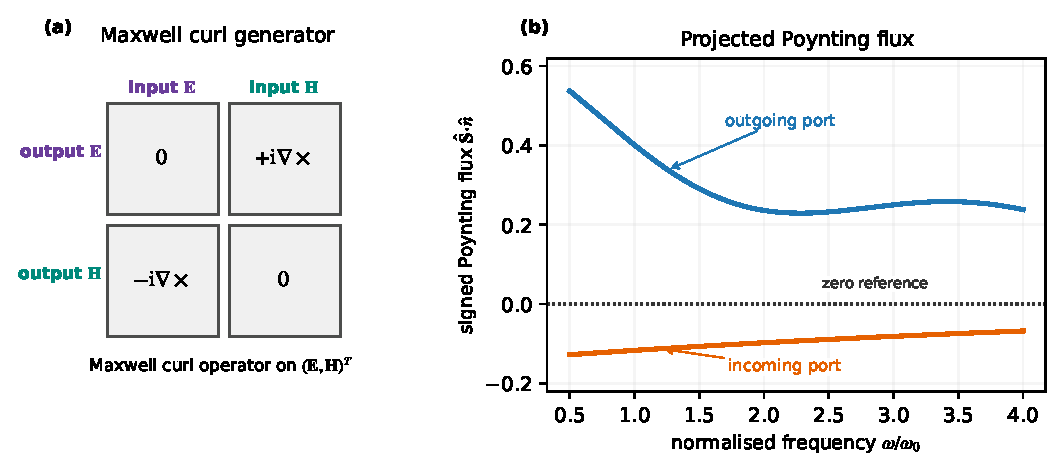
\includegraphics[width=0.92\textwidth]{figures/fig_ch02_operator_structure_step199.pdf}
  \caption{Structure of the Maxwell curl operator $\Maxop$ and energy flux.
  \textbf{(a)}~Block structure of the time generator: the $6\times 6$
  operator $\Maxop$ defined in \eqref{eq:ch2-maxop} has vanishing diagonal
  blocks (no direct $\Efield$--$\Efield$ or $\Hfield$--$\Hfield$ coupling)
  and antisymmetric off-diagonal curl blocks ($+\ii\nabla\times$ couples
  $\Hfield$ into the $\Efield$ equation; $-\ii\nabla\times$ couples
  $\Efield$ into the $\Hfield$ equation), consistent with the
  $e^{-\ii\omega t}$ time convention used throughout this book.
  \textbf{(b)}~Signed normal Poynting flux $\hat{\mathbf{S}}\cdot\hat{n}$
  for a guided mode at a port boundary, illustrating energy flow into
  (incoming port) and out of (outgoing port) the computational domain.
  The zero reference line marks the interface between forward and
  backward flux.}
  \label{fig:ch02-operator-structure}
\end{figure}


\begin{remark}
The off-diagonal structure of $\Maxop$ in
\eqref{eq:ch2-maxop}---coupling $\Efield$ to $\Hfield$ through the
curl---is a reflection of the fact that electromagnetic waves are
intrinsically coupled electric and magnetic phenomena.  This structure
is preserved under all linear constitutive extensions and is the origin
of the spin-1 character of photons.
\end{remark}

\subsection{Momentum representation}
\label{sec:ch2-momentum}

For a spatially homogeneous medium, or for the cell-periodic part of a
Bloch mode in a periodic medium, we can replace $\nabla$ by
$\ii\kvec$ to obtain the momentum-space curl operator
\begin{equation}\label{eq:ch2-maxop-k}
  \Maxop(\kvec)
  =
  \begin{pmatrix}
    \mathbf{0} & -\kvec\times \\[2pt]
    \kvec\times & \mathbf{0}
  \end{pmatrix},
\end{equation}
where $(\kvec\times)_{ij}=-\epsilon_{ijk}k_k$ is the $3\times 3$
antisymmetric matrix associated with the cross product.  Explicitly, for
$\kvec=(k_x,k_y,k_z)$:
\begin{equation}\label{eq:ch2-cross-matrix}
  \kvec\times
  =
  \begin{pmatrix}
    0 & -k_z & k_y \\
    k_z & 0 & -k_x \\
    -k_y & k_x & 0
  \end{pmatrix}.
\end{equation}
It is straightforward to verify that $\Maxop(\kvec)$ is Hermitian:
$\Maxop(\kvec)=\Maxop^\dagger(\kvec)$, since the cross-product matrix
is real and antisymmetric, so $(\kvec\times)^T=-\kvec\times$, and the
block off-diagonal structure with the signs in \eqref{eq:ch2-maxop-k}
makes the full $6\times6$ matrix symmetric.

\begin{remark}[Spin-1 matrices]
Haldane and Raghu write the curl operator as $A=-\ii J^a\nabla_a$,
where $J^a$ are $6\times6$ matrices built from the spin-1
representation of $\mathrm{SO}(3)$.  In components,
$(L^a)_{bc}=\ii\epsilon_{abc}$ are the $3\times3$ generators of
rotations, and $J^a$ is the block off-diagonal matrix
$J^a = \bigl(\begin{smallmatrix}0 & \ii L^a \\ -\ii L^a &
0\end{smallmatrix}\bigr)$.  This representation makes the rotational
symmetry of the Maxwell operator manifest and connects directly to the
spin-1 nature of the photon.
\end{remark}


\section{Electromagnetic energy}
\label{sec:ch2-energy}

The energy carried by electromagnetic fields is central to everything
that follows.  The correct inner product for the Maxwell eigenvalue
problem is built from the electromagnetic energy, so we derive the
Poynting theorem in detail.

\subsection{Poynting's theorem in the time domain}
\label{sec:ch2-poynting-time}

We start from the standard derivation.  Take the dot product of
\eqref{eq:ch2-faraday} with $\Hfield$ and of \eqref{eq:ch2-ampere}
with $\Efield$:
\begin{align}
  \Hfield\cdot(\nabla\times\Efield)
  &= -\Hfield\cdot\pderiv{\Bfield}{t}\,,
  \label{eq:ch2-poynting-step1}\\
  \Efield\cdot(\nabla\times\Hfield)
  &= \Efield\cdot\pderiv{\Dfield}{t}\,.
  \label{eq:ch2-poynting-step2}
\end{align}
Subtract \eqref{eq:ch2-poynting-step1} from
\eqref{eq:ch2-poynting-step2} and use the vector identity
$\nabla\cdot(\Efield\times\Hfield)
 =\Hfield\cdot(\nabla\times\Efield)
 -\Efield\cdot(\nabla\times\Hfield)$
to obtain
\begin{equation}\label{eq:ch2-poynting-differential}
  \nabla\cdot(\Efield\times\Hfield)
  + \Efield\cdot\pderiv{\Dfield}{t}
  + \Hfield\cdot\pderiv{\Bfield}{t}
  = 0\,.
\end{equation}
Define the Poynting vector and the instantaneous energy density:
\begin{equation}\label{eq:ch2-poynting-defs}
  \Sfield(\rvec,t) = \Efield\times\Hfield\,,
  \qquad
  u(\rvec,t) = \frac{1}{2}\bigl(
    \Efield\cdot\Dfield + \Hfield\cdot\Bfield
  \bigr).
\end{equation}
For nondispersive media with $\Dfield=\varepsilon_0\epst\Efield$ and \cite{silveirinha2016bulk}
$\Bfield=\mu_0\mut\Hfield$, the terms
$\Efield\cdot\partial_t\Dfield$ and $\Hfield\cdot\partial_t\Bfield$
equal $\partial_t u$ when $\epst$ and $\mut$ are
time-independent.\footnote{%
  For dispersive media the identification
  $\Efield\cdot\partial_t\Dfield=\partial_t(\frac12\Efield\cdot\Dfield)$
  does not hold in general; see \secref{sec:ch2-dispersive-energy}.}
Poynting's theorem then takes the conservation-law form
\begin{equation}\label{eq:ch2-poynting-conservation}
  \boxed{%
  \pderiv{u}{t} + \nabla\cdot\Sfield = 0\,.}
\end{equation}
Integrating over any volume $V$ bounded by a surface $\partial V$:
\begin{equation}
  \tderiv{}{t}\int_V u\,\dd^3r
  = -\oint_{\partial V}\Sfield\cdot\hat{n}\,\dd A\,.
\end{equation}
Energy stored in $V$ changes only through the Poynting flux across the
boundary.  In a lossless medium, energy is neither created nor
destroyed; the field energy is exactly accounted for by the flux.

\subsection{Time-averaged energy for harmonic fields}
\label{sec:ch2-energy-harmonic}

For monochromatic fields
$\Efield(\rvec,t)=\real[\Efield(\rvec)\ee^{-\ii\omega t}]$, the
time-averaged Poynting vector and energy density are
\begin{equation}\label{eq:ch2-time-avg}
  \langle\Sfield\rangle
  = \frac{1}{2}\real(\Efield\times\Hfield^*)\,,
  \qquad
  \langle u\rangle
  = \frac{1}{4}\real\bigl(
    \Efield^*\cdot\Dfield + \Hfield^*\cdot\Bfield
  \bigr).
\end{equation}

Using the bianisotropic constitutive relation \eqref{eq:ch2-bianisotropic},
the time-averaged energy density can be written compactly in terms of
the six-component field as
\begin{equation}\label{eq:ch2-energy-sixfield}
  \langle u\rangle
  = \frac{1}{4}\,\emfield^\dagger(\rvec)\cdot\Mmat(\rvec,\omega)
    \cdot\emfield(\rvec)\,.
\end{equation}
When $\Mmat$ is Hermitian and positive definite, $\langle u\rangle>0$
for any nonzero $\emfield$.  This is the physical content of
Definitions~\ref{def:ch2-lossless} and \ref{def:ch2-positive-energy}.

\subsection{Energy in dispersive media}
\label{sec:ch2-dispersive-energy}

All real materials are dispersive: the material matrix
$\Mmat(\rvec,\omega)$ depends on frequency.  In a dispersive
medium, the time-averaged energy density of a \emph{quasi-monochromatic}
wave packet (bandwidth $\Delta\omega\ll\omega$) is given by the
Brillouin formula
\begin{equation}\label{eq:ch2-brillouin-energy}
  \langle u\rangle_{\mathrm{disp}}
  = \frac{1}{4}\,\emfield^\dagger(\rvec)\cdot
  \pderiv{}{\omega}\bigl[\omega\,\Mmat(\rvec,\omega)\bigr]
  \cdot\emfield(\rvec)
  = \frac{1}{4}\,\emfield^\dagger\cdot\Mgmat(\omega)\cdot\emfield\,,
\end{equation}
where we define the \emph{energy metric}
\begin{equation}\label{eq:ch2-energy-metric}
  \boxed{%
  \Mgmat(\rvec,\omega)
  \;\equiv\;
  \pderiv{}{\omega}\bigl[\omega\,\Mmat(\rvec,\omega)\bigr]
  = \Mmat + \omega\,\pderiv{\Mmat}{\omega}\,.}
\end{equation}

\begin{remark}
In the nondispersive limit ($\partial\Mmat/\partial\omega=0$), the
energy metric reduces to $\Mgmat=\Mmat$, and
\eqref{eq:ch2-brillouin-energy} reduces to
\eqref{eq:ch2-energy-sixfield}.
\end{remark}

The requirement that the electromagnetic energy is positive
($\langle u\rangle_\mathrm{disp}>0$ for all nonzero $\emfield$)
translates into the \emph{stability condition}:
\begin{equation}\label{eq:ch2-stability}
  \Mgmat(\rvec,\omega)\;\text{is positive definite}
\end{equation}
at every physical eigenfrequency.  This condition was emphasised by
Haldane and Raghu as the correct generalisation of the positive-energy
requirement for dispersive Maxwell systems, and it will play a crucial
role in the inner product of \chref{ch:normal-modes}.

\paragraph{Derivation of the Brillouin formula.}
The result \eqref{eq:ch2-brillouin-energy} can be derived by
considering a wave packet
$\Efield(\rvec,t)=\real[\hat\Efield(\rvec)\,a(t)\,\ee^{-\ii\omega_0 t}]$
with slowly varying envelope $a(t)$ centred at frequency $\omega_0$.
The constitutive relation in the time domain involves a convolution:
$\Dfield(\rvec,t)=\int_{-\infty}^{t}\varepsilon_0\epst(\rvec,t-t')
\Efield(\rvec,t')\,\dd t'$.  For a narrow-band envelope, one expands
the frequency-domain susceptibility to first order around $\omega_0$:
\begin{equation}
  \omega\,\varepsilon_{ij}(\omega)
  \approx \omega_0\,\varepsilon_{ij}(\omega_0)
  + (\omega-\omega_0)\,
  \pderiv{}{\omega}\bigl[\omega\,\varepsilon_{ij}\bigr]
  \Big|_{\omega_0}.
\end{equation}
Substituting into the Poynting identity and time-averaging over the
carrier oscillation yields \eqref{eq:ch2-brillouin-energy} for the
$\epst$ block; the $\mut$, $\xit$, and $\zetat$ blocks follow
identically, giving the full $6\times 6$ result.

\section{Poynting's theorem for harmonic fields}
\label{sec:ch2-poynting}

We now derive the frequency-domain version of Poynting's theorem and
show that it encodes the losslessness condition directly.

Take the complex conjugate of \eqref{eq:ch2-faraday-freq}:
$\nabla\times\Efield^*=-\ii\omega\Bfield^*$.  Form
$\Hfield\cdot(\nabla\times\Efield^*)-\Efield^*\cdot(\nabla\times\Hfield)$
and use the identity
$\nabla\cdot(\Efield^*\times\Hfield)
=\Hfield\cdot(\nabla\times\Efield^*)
-\Efield^*\cdot(\nabla\times\Hfield)$:
\begin{equation}\label{eq:ch2-complex-poynting}
  \nabla\cdot(\Efield^*\times\Hfield)
  = -\ii\omega\bigl(
    \Hfield\cdot\Bfield^* - \Efield^*\cdot\Dfield
  \bigr).
\end{equation}
Using the constitutive relation in six-component form, the right-hand
side becomes
\begin{equation}
  -\ii\omega\,\emfield^\dagger
  \begin{pmatrix}
    -\vac\epst & -\clight^{-1}\xit \\
    \muvac\mut^\dagger & \clight^{-1}\zetat^\dagger
  \end{pmatrix}
  \emfield\,.
\end{equation}
Taking the imaginary part:
\begin{equation}\label{eq:ch2-loss-condition}
  \frac{1}{2}\nabla\cdot\real(\Efield^*\times\Hfield)
  = -\frac{\omega}{2}\,\emfield^\dagger\cdot
    \frac{\Mmat-\Mmat^\dagger}{2\ii}\cdot\emfield\,.
\end{equation}
The left-hand side is the divergence of the time-averaged Poynting
vector.  If $\Mmat=\Mmat^\dagger$, the right-hand side vanishes
identically: the divergence of the Poynting flux is zero everywhere,
confirming that no energy is absorbed or generated.

\begin{proposition}[Losslessness from Hermiticity]
  \label{prop:ch2-lossless}
  A linear medium is lossless (zero absorption and gain at frequency
  $\omega$) if and only if $\Mmat(\rvec,\omega)=\Mmat^\dagger(\rvec,\omega)$.
\end{proposition}

\section{Symmetries of the Maxwell system}
\label{sec:ch2-symmetries}

The topological classification of photonic bands depends critically on
which discrete symmetries the Maxwell system possesses \cite{ozawa2018topological}.  We now derive
the three most important ones from the structure of $\Mmat$ and
$\Maxop$.

\subsection{Time reversal}
\label{sec:ch2-time-reversal}

The microscopic Maxwell equations are invariant under time reversal
$t\to -t$.  In the macroscopic theory, time reversal acts on the fields
as
\begin{equation}\label{eq:ch2-TR-fields}
  \Top:\;
  \Efield(\rvec,t)\to\Efield(\rvec,-t)\,,\quad
  \Hfield(\rvec,t)\to-\Hfield(\rvec,-t)\,.
\end{equation}
The sign difference arises because $\Efield$ is a polar vector
(unchanged under $t\to -t$) while $\Hfield$ is an axial vector
proportional to a current ($\Jfield\propto\dd q/\dd t$ changes sign).

For a time-harmonic field $\emfield\ee^{-\ii\omega t}$, the
time-reversal operation becomes complex conjugation combined with a sign
flip on the magnetic component:
\begin{equation}\label{eq:ch2-TR-harmonic}
  \Top:\;
  \begin{pmatrix}\Efield\\\Hfield\end{pmatrix}
  \;\mapsto\;
  \begin{pmatrix}\Efield^*\\-\Hfield^*\end{pmatrix},
  \qquad
  \kvec\to-\kvec\,,\quad \omega\to\omega\,.
\end{equation}
We can represent this as $\Top=\mathcal{K}\,\sigma_z$, where
$\mathcal{K}$ is complex conjugation and
$\sigma_z=\diag(\mathbf{I}_3,-\mathbf{I}_3)$ acts on the
electric/magnetic block structure.

\paragraph{Bosonic time reversal: $\Top^2=+1$.}
Applying $\Top$ twice:
$\Top^2\emfield = \mathcal{K}\sigma_z\mathcal{K}\sigma_z\emfield
= \sigma_z^2\emfield = \emfield$.
Thus $\Top^2=+\mathbf{1}$ for photons.  This is fundamentally different
from the electronic case, where $\Top^2=-\mathbf{1}$ due to half-integer
spin.

\begin{proposition}[Absence of photonic Kramers degeneracy]
  \label{prop:ch2-no-kramers}
  Since $\Top^2=+1$ for photons, there is no Kramers theorem for
  electromagnetic modes.  Time-reversal symmetry alone does not
  guarantee twofold degeneracy at time-reversal-invariant momenta.
  Consequently, the $\mathbb{Z}_2$ topological classification of the
  quantum spin Hall effect does not directly apply to photonic systems.
\end{proposition}

\paragraph{Condition on the material matrix.}
The Maxwell eigenvalue equation is time-reversal invariant if and only
if, for every solution $\emfield$ at $(\omega,\kvec)$, the
time-reversed field $\Top\emfield$ is also a solution at
$(\omega,-\kvec)$.  Substituting into \eqref{eq:ch2-maxwell-matrix} and
using the explicit form of $\Top$, one finds that this requires
\begin{equation}\label{eq:ch2-TR-condition}
  \sigma_z\,\Mmat^*(\omega)\,\sigma_z = \Mmat(\omega)\,.
\end{equation}
In block form, this reads
\begin{equation}\label{eq:ch2-TR-blocks}
  \epst^* = \epst\,,\quad
  \mut^* = \mut\,,\quad
  \xit^* = -\xit\,,\quad
  \zetat^* = -\zetat\,.
\end{equation}
For the gyrotropic permeability of \eqref{eq:ch2-gyrotropic-mu},
condition \eqref{eq:ch2-TR-blocks} requires $\kappa=0$.  A nonzero
gyrotropic parameter therefore \emph{breaks time-reversal symmetry}.

\subsection{Reciprocity}
\label{sec:ch2-reciprocity}

A medium is \emph{reciprocal} if the Lorentz reciprocity relation holds:
for any two solutions $\emfield_a$ and $\emfield_b$ of the Maxwell
equations at the same frequency,
\begin{equation}
  \int_V\bigl(
    \Efield_a\cdot\Jfield_b - \Efield_b\cdot\Jfield_a
  \bigr)\dd^3r = 0\,
\end{equation}
The displayed formula above follows the convention and normalisation used in \cite{v2024exact}.
In terms of the material matrix, reciprocity requires
\begin{equation}\label{eq:ch2-reciprocity}
  \epst = \epst^T\,,\quad
  \mut = \mut^T\,,\quad
  \xit = -\zetat^T\,.
\end{equation}

\begin{proposition}[Equivalence of TR symmetry and reciprocity for
  lossless media]
  \label{prop:ch2-TR-reciprocal}
  For a lossless medium ($\Mmat=\Mmat^\dagger$), the time-reversal
  condition \eqref{eq:ch2-TR-blocks} is equivalent to the reciprocity
  condition \eqref{eq:ch2-reciprocity}.
\end{proposition}

\begin{proof}
For a Hermitian tensor, $\epst=\epst^\dagger$ means
$\varepsilon_{ij}=\varepsilon_{ji}^*$.  The TR condition
$\epst^*=\epst$ means $\varepsilon_{ij}^*=\varepsilon_{ij}$, so
$\varepsilon_{ij}$ is real, which combined with Hermiticity gives
$\varepsilon_{ij}=\varepsilon_{ji}=\epst^T$---precisely reciprocity.
The argument for $\mut$ is identical.  For the coupling tensors:
Hermiticity gives $\zetat=\xit^\dagger$; the TR condition
$\xit^*=-\xit$ means $\xit$ is pure imaginary.  Then
$\xit^\dagger=\xit^{*T}=-\xit^T$, so
$\zetat=\xit^\dagger=-\xit^T$, which is the reciprocity condition.
The converse follows by reversing the steps.
\end{proof}

The physical content of this result is that, for lossless photonic
systems, the route to nonzero Chern numbers and one-way edge states
runs through \emph{nonreciprocal} media---media that violate both
TR symmetry and Lorentz reciprocity.  The gyrotropic ferrites
used in the first topological photonic-crystal experiments are the
prototypical example.

\subsection{Spatial inversion}
\label{sec:ch2-inversion}

The inversion (parity) operator $\Pop$ acts as
\begin{equation}\label{eq:ch2-inversion}
  \Pop:\;
  \Efield(\rvec)\to-\Efield(-\rvec)\,,\quad
  \Hfield(\rvec)\to\Hfield(-\rvec)\,,\quad
  \kvec\to-\kvec\,.
\end{equation}
The signs follow from the polar/axial character of the fields under
$\rvec\to-\rvec$.  In the six-component notation,
$\Pop = -\sigma_z\,\hat{P}_\rvec$, where $\hat{P}_\rvec$ sends
$\rvec\to-\rvec$.

The Maxwell system is inversion-symmetric if
$\Mmat(-\rvec,\omega)=\sigma_z\,\Mmat(\rvec,\omega)\,\sigma_z$.
When both $\Top$ and $\Pop$ are present, the combined symmetry
$\Top\Pop$ maps $(\omega,\kvec)$ to $(\omega,\kvec)$ and constrains
the Berry curvature to vanish identically at every $\kvec$ point
(see \chref{ch:geometry-bands}).

\section{The road ahead}
\label{sec:ch2-road-ahead}

We have now assembled the raw materials: the Maxwell equations in
first-order six-component form, the material matrix encoding all linear
constitutive information, the Poynting theorem guaranteeing energy
conservation, and the discrete symmetries that will control the
topological classification.

What is still missing is the \emph{mode structure}.  The eigenvalue
equation \eqref{eq:ch2-maxwell-matrix} determines a set of normal modes
at each frequency and wavevector, but we have not yet shown that these
modes are orthogonal, how they are normalised, or what inner product
makes the problem self-adjoint.  These are the questions of the next
chapter.

\section{Hamiltonian structure of the Maxwell system}
\label{sec:ch2-hamiltonian}

The first-order Maxwell system \eqref{eq:ch2-maxwell-matrix} has a
natural Hamiltonian structure that is worth making explicit, because
it connects the photonic eigenvalue problem to the broader framework
of symplectic dynamics and provides additional insight into why the
Berry phase is a geometric quantity.

\subsection{Symplectic form and Poisson bracket}
\label{sec:ch2-symplectic}

Define the symplectic matrix
$\mathbf{J}=\bigl(\begin{smallmatrix}0&-\mathbf{I}_3\\
\mathbf{I}_3&0\end{smallmatrix}\bigr)$ and the electromagnetic
energy density $\mathcal{U}=\frac{1}{2}\emfield^\dagger\Mmat\emfield$.
Then the source-free Maxwell equations can be written as
\begin{equation}\label{eq:ch2-symplectic-form}
  \Mmat\,\partial_t\emfield
  = \mathbf{J}\,\nabla\times\emfield\,,
\end{equation}
which is a Hamiltonian system with ``coordinates''
$(\Efield,\Hfield)$ and ``Hamiltonian functional''
$\mathcal{H}[\emfield]=\int\mathcal{U}\,\dd^3 r$.  The symplectic
structure is encoded in $\mathbf{J}$, and the material matrix $\Mmat$
plays the role of a metric on the phase space.

For a lossless medium ($\Mmat=\Mmat^\dagger$, positive definite),
the Hamiltonian $\mathcal{H}$ is conserved (the Poynting theorem),
and the eigenfrequencies are real.  For a lossy medium, the
anti-Hermitian part of $\Mmat$ produces dissipation, the
eigenfrequencies acquire imaginary parts, and the system moves into the
non-Hermitian territory of Chapter~\ref{ch:non-hermitian}
\cite{ozawa2018topological}.

\subsection{The positive-definite condition}
\label{sec:ch2-positive-definite}

The requirement that $\Mmat$ be positive definite is the mathematical
expression of the physical condition that the electromagnetic energy
density $\mathcal{U}=\frac{1}{2}\emfield^\dagger\Mmat\emfield$ be
positive for all nonzero field configurations.  This condition is
satisfied by all passive dielectric and magnetic materials at
frequencies below any resonance.

Near a material resonance (e.g., the ferromagnetic resonance in YIG
at $\omega_0$, Chapter~\ref{ch:microwave-crystal}), one or more
eigenvalues of $\Mmat(\omega)$ pass through zero and become negative.
In these regimes, the non-dispersive energy density is no longer
positive definite, and one must use the dispersive energy metric
$\Mgmat(\omega)=\partial_\omega[\omega\Mmat(\omega)]$ introduced in
Chapter~\ref{ch:normal-modes}.  The dispersive metric remains
positive definite as long as the material is passive, by virtue of
the Kramers--Kronig relations (Appendix~\ref{app:material-tensors})
\cite{gangaraj2016berry,silveirinha2016bulk}.

\subsection{Phase-space volume and Liouville's theorem}
\label{sec:ch2-liouville}

In a conservative Hamiltonian system, Liouville's theorem guarantees
conservation of phase-space volume.  For the electromagnetic system,
this translates into the statement that the eigenvalue spectrum is
stable under perturbations that preserve the lossless condition: real
eigenfrequencies cannot ``collide and annihilate'' unless a symmetry
allows it (the von Neumann--Wigner codimension argument of
Chapter~\ref{ch:dirac-cones}).

When loss is introduced, the Liouville structure breaks down and
eigenfrequencies can coalesce at exceptional points, producing the
rich non-Hermitian physics discussed in
Chapter~\ref{ch:non-hermitian} \cite{price2022roadmap}.

\section{Lorentz reciprocity from Maxwell's equations}
\label{sec:ch2-reciprocity-lorentz}

Lorentz reciprocity is a fundamental symmetry of Maxwell's equations
that has profound implications for topological photonics.  The
reciprocity theorem states that for two sets of sources
$(\Jfield_1,\Jfield_2)$ producing fields
$(\Efield_1,\Hfield_1)$ and $(\Efield_2,\Hfield_2)$ in the same
medium, the reaction integrals are equal:
\begin{equation}\label{eq:ch2-lorentz-reciprocity}
  \int\bigl(\Efield_1\cdot\Jfield_2
  - \Hfield_1\cdot\mathbf{M}_2\bigr)\,\dd^3 r
  = \int\bigl(\Efield_2\cdot\Jfield_1
  - \Hfield_2\cdot\mathbf{M}_1\bigr)\,\dd^3 r\,,
\end{equation}
where $\mathbf{M}_a$ are magnetic current sources.

\subsection{Derivation from the material symmetry}
\label{sec:ch2-reciprocity-derivation}

The proof proceeds by writing Maxwell's equations for both source
configurations and forming the divergence
$\nabla\cdot(\Efield_1\times\Hfield_2-\Efield_2\times\Hfield_1)$.
Expanding via the vector identity and substituting the frequency-domain
Maxwell equations \eqref{eq:ch2-maxwell-freq}, the surface integral
vanishes for sources of compact support, leaving:
\begin{equation}\label{eq:ch2-reciprocity-condition}
  \ii\omega\int\bigl[
    \Efield_1\!\cdot\!(\varepsilon^T\!-\!\varepsilon)\Efield_2
    + \Hfield_1\!\cdot\!(\mu^T\!-\!\mu)\Hfield_2
    + \Efield_1\!\cdot\!(\zeta^T\!+\!\xi)\Hfield_2
    - \Efield_2\!\cdot\!(\zeta^T\!+\!\xi)\Hfield_1
  \bigr]\dd^3 r = 0\,.
\end{equation}
Crucially, this bilinear form involves the \emph{unconjugated}
transpose (not the Hermitian conjugate), because the Lorentz identity
is linear in the fields.  The integrand vanishes for all field
configurations if and only if the material tensors satisfy the block
conditions
\begin{equation}\label{eq:ch2-block-reciprocity}
  \varepsilon = \varepsilon^T\,,\qquad
  \mu = \mu^T\,,\qquad
  \xi = -\zeta^T\,
\end{equation}
The displayed formula above follows the convention and normalisation used in \cite{wang2007reflection}.
These are the Lorentz reciprocity conditions for bianisotropic media.
Note that the full $6\times 6$ material matrix $\Mmat$ is
\emph{not} required to be symmetric; instead, the off-diagonal blocks
satisfy the antisymmetry condition $\xi=-\zeta^T$.  For a gyrotropic
medium with $\kappa_\mu\neq 0$, the permeability tensor
$\mu\neq\mu^T$, and reciprocity is broken---the essential prerequisite
for a photonic Chern insulator
\cite{ozawa2018topological,gangaraj2016berry}.

\subsection{Implications for topology}
\label{sec:ch2-reciprocity-topology}

The breaking of reciprocity is intimately connected to the breaking
of time-reversal symmetry: a reciprocal medium satisfies
$\Mmat=\Mmat^T$, which is equivalent to $\Top$-invariance of the
Maxwell eigenproblem.  Since $\Top$-invariance forces
$\Chern_n=0$ (Chapter~\ref{ch:geometry-bands}), a nonreciprocal
medium is a necessary condition for a photonic Chern insulator.

Conversely, a photonic topological insulator with $\Top$-symmetry
(Chapter~\ref{ch:reciprocal-designs}) must be reciprocal, and its
topology is protected by spatial symmetries rather than by the Chern
number.  This dichotomy---Chern insulators require nonreciprocity,
while $\mathbb{Z}_2$ and crystalline phases are reciprocal---organises
the entire field of topological photonics
\cite{haldane2008possible,price2022roadmap}.

\section{Energy density and energy velocity}
\label{sec:ch2-energy-velocity}

The time-averaged energy density stored in a monochromatic field
at frequency $\omega$ in a dispersive medium is the Brillouin energy
density \cite{gangaraj2016berry,silveirinha2016bulk}:
\begin{equation}\label{eq:ch2-brillouin-energy-density}
  \langle\mathcal{U}\rangle
  = \frac{1}{4}\emfield^\dagger\,
  \frac{\partial[\omega\Mmat(\omega)]}{\partial\omega}\,\emfield
  = \frac{1}{4}\emfield^\dagger\Mgmat(\omega)\,\emfield\,.
\end{equation}
The energy velocity is defined as the ratio of the time-averaged
Poynting flux to the energy density:
$\mathbf{v}_E=\langle\mathbf{S}\rangle/\langle\mathcal{U}\rangle$.

For a lossless, non-dispersive medium, the energy velocity equals
the group velocity.  For a dispersive medium, the two can differ near
material resonances, but they agree in the transparency windows where
$\imag\,\Mmat\approx 0$.  The energy velocity is always bounded by
$c$ in a passive medium, which provides a physical check on numerical
computations of photonic band structures.

The dispersive energy metric $\Mgmat(\omega)$ is the key quantity
that connects energy conservation, the electromagnetic inner product
(Chapter~\ref{ch:normal-modes}), and the Berry geometry
(Chapter~\ref{ch:geometry-bands}).

\section{Energy conservation and the Maxwell generator}
\label{sec:ch2-energy-generator-detail}

The compact equation $\Maxop\Psi=\ii\partial_t(\Mmat\Psi)$ is useful
only if it carries the ordinary physical meaning of Maxwell's
equations.  Let us verify explicitly that the operator form reproduces
Poynting's theorem and identifies the correct Hilbert-space metric.
For a source-free, lossless, nondispersive medium with Hermitian
$\varepsilon$ and $\mu$, Maxwell's equations are
\begin{equation}\label{eq:ch2-time-domain-maxwell-pair}
  \nabla\times\Efield=-\partial_t\Bfield,
  \qquad
  \nabla\times\Hfield=\partial_t\Dfield,
  \qquad
  \Dfield=\varepsilon\Efield,
  \quad
  \Bfield=\mu\Hfield.
\end{equation}
Take the scalar product of the second equation with $\Efield^*$ and
of the first equation with $\Hfield^*$, subtract the complex conjugate
identity where needed, and use
\begin{equation}\label{eq:ch2-poynting-vector-identity}
  \nabla\cdot(\Efield\times\Hfield^*)
  = \Hfield^*\cdot(\nabla\times\Efield)
    -\Efield\cdot(\nabla\times\Hfield^*).
\end{equation}
For real time-domain fields this gives the local conservation law
\begin{equation}\label{eq:ch2-poynting-theorem-local}
  \partial_t u + \nabla\cdot\Sfield =0,
  \qquad
  u=\frac{1}{2}\bigl(\Efield\cdot\Dfield+
  \Hfield\cdot\Bfield\bigr),
  \qquad
  \Sfield=\Efield\times\Hfield.
\end{equation}
Thus the quadratic form associated with the material matrix is not an
arbitrary mathematical choice; it is the electromagnetic energy.  For a
mode in a closed cavity or a Bloch mode integrated over a unit cell, the
conserved norm is
\begin{equation}\label{eq:ch2-conserved-maxwell-norm}
  \|\Psi\|^2_{\Mmat}
  = \int \Psi^\dagger\Mmat\Psi\,\dd^3r
  = \int \bigl(\Efield^*\cdot\varepsilon\Efield
  +\Hfield^*\cdot\mu\Hfield\bigr)\,\dd^3r.
\end{equation}

This calculation explains why the Maxwell generator is self-adjoint in
the energy metric rather than in the flat field metric.  If
$\hat{H}_{\mathrm{M}}=\Mmat^{-1}\Maxop$ and the boundary term
$\int_{\partial V}\hat{n}\cdot(\Efield_1^*\times\Hfield_2)\,\dd A$
vanishes because of periodic, PEC, or radiation-compatible boundary
conditions, then
\begin{equation}\label{eq:ch2-generator-selfadjoint}
  \langle \Psi_1,\hat{H}_{\mathrm{M}}\Psi_2\rangle_{\Mmat}
  =\langle \hat{H}_{\mathrm{M}}\Psi_1,\Psi_2\rangle_{\Mmat}.
\end{equation}
The eigenfrequencies are therefore real, and eigenmodes at different
frequencies are orthogonal in the energy inner product
\cite{raghu2008analogs}.  This is the
Maxwell analogue of Hermiticity in quantum mechanics, but its origin is
Poynting's theorem, not probability conservation.

\section{What changes in a dispersive material}
\label{sec:ch2-dispersive-energy-preview}

Topological photonic media are often strongly dispersive.  Ferrites,
plasmas, metamaterials, and resonator arrays all acquire their useful
band gaps from internal material or structural resonances.  In such a
medium the naive energy density
$\frac{1}{2}(\Efield\cdot\Dfield+\Hfield\cdot\Bfield)$ is not the
stored energy of a monochromatic wave, because some energy resides in
the microscopic polarisation or magnetisation degrees of freedom.
For a lossless linear medium with frequency-domain material matrix
$\Mmat(\omega)$, the correct cycle-averaged energy density is
\begin{equation}\label{eq:ch2-brillouin-energy-preview}
  u_\omega
  =\frac{1}{4}\Psi^\dagger
  \partial_\omega\bigl[\omega\Mmat(\omega)\bigr]\Psi.
\end{equation}
The matrix
$\Mgmat(\omega)=\partial_\omega[\omega\Mmat(\omega)]$ is positive in a
transparent frequency window of a passive medium.  Positivity is not a
technical assumption; it is the statement that a finite-amplitude field
stores positive energy in both the electromagnetic field and the bound
material oscillators.

This observation will be used repeatedly.  In Chapter~\ref{ch:normal-modes}
it becomes the orthogonality metric for dispersive Maxwell modes.  In
Chapter~\ref{ch:geometry-bands} it becomes the metric used to normalise
Bloch modes before Berry curvature is computed.  In Chapter~\ref{ch:microwave-crystal}
it is the reason the gyromagnetic YIG bands can be assigned Chern
numbers only in a frequency window separated from ferromagnetic
resonance loss.  The word ``topological'' never removes the need to
ask where the electromagnetic energy is stored.

\begin{figure}[t]
  \centering
  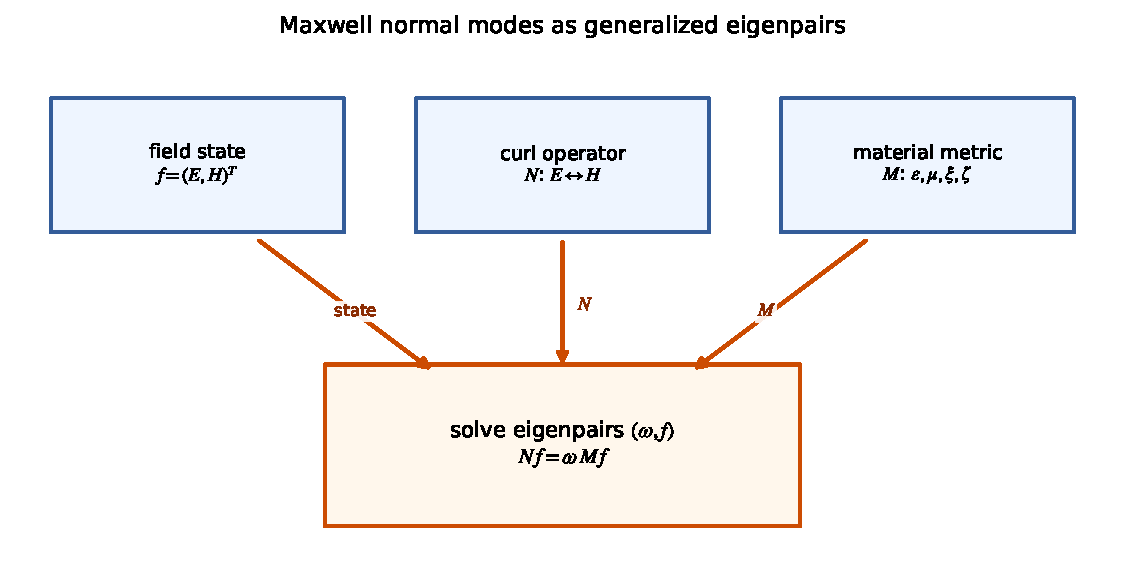
\includegraphics[width=0.88\textwidth]{figures/fig_ch02_maxwell_blocks.pdf}
  \caption{Maxwell's equations as a six-component normal-mode problem.
  The electromagnetic field state $\mathbf{f}=(\mathbf{E},\mathbf{H})^T$
  is acted on by the curl operator $N$, while the material tensor $M$
  supplies the energy metric.  Topological band theory for photons starts
  only after this metric structure is fixed.}
  \label{fig:ch02-maxwell-blocks}
\end{figure}

\section*{Exercises}

\begin{exercise}
  Verify by direct computation that the $6\times6$ momentum-space curl
  operator $\Maxop(\kvec)$ defined in \eqref{eq:ch2-maxop-k} is
  Hermitian.  \emph{Hint:} write out the full matrix for a general
  $\kvec=(k_x,k_y,k_z)$ and check that it equals its conjugate
  transpose.
\end{exercise}

\begin{exercise}
  For an isotropic medium with scalar $\varepsilon$ and $\mu$, show
  that the eigenvalues of the $6\times 6$ matrix
  $\Mmat^{-1}\Maxop(\kvec)$ are
  $\omega=\pm|\kvec|/\sqrt{\varepsilon_0\mu_0\varepsilon\mu}$
  (each twofold degenerate, corresponding to two transverse
  polarisations) and $\omega=0$ (twofold, corresponding to
  longitudinal modes).  Identify the physical content of each.
\end{exercise}

\begin{exercise}
  The gyrotropic permeability tensor \eqref{eq:ch2-gyrotropic-mu} has
  eigenvalues $\mu_\perp\pm\kappa$ for circular polarisations and
  $\mu_z$ for the $z$-component.  Derive the two circular-polarisation
  refractive indices $n_\pm=\sqrt{\varepsilon(\mu_\perp\pm\kappa)}$
  for a plane wave propagating along $\hat{z}$ in a medium with scalar
  permittivity $\varepsilon$ and gyrotropic permeability.  Show that
  the Faraday rotation per unit length is
  $\theta_F=\omega(n_+-n_-)/(2c)$.
\end{exercise}

\begin{exercise}
  Prove that the complex Poynting identity
  \eqref{eq:ch2-complex-poynting} holds by starting from the curl
  equations \eqref{eq:ch2-maxwell-freq} and using the vector identity
  $\nabla\cdot(\mathbf{A}\times\mathbf{B})
  =\mathbf{B}\cdot(\nabla\times\mathbf{A})
  -\mathbf{A}\cdot(\nabla\times\mathbf{B})$.
\end{exercise}

\begin{exercise}
  Show that for a lossless nondispersive medium, the divergence of the
  time-averaged Poynting vector vanishes:
  $\nabla\cdot\langle\Sfield\rangle=0$.  What additional condition is
  needed for this to hold in a dispersive medium?
\end{exercise}

\begin{exercise}
  Starting from the bianisotropic constitutive relation
  \eqref{eq:ch2-bianisotropic}, verify explicitly that the
  time-reversal condition \eqref{eq:ch2-TR-condition} applied to
  $\Mmat$ yields the block conditions \eqref{eq:ch2-TR-blocks}.
\end{exercise}
